\section{Evaluation, Conclusions and Future Work}
\subsection{Project Objectives}
As a result of the project, a few things were made:
\begin{enumerate}
    \item Collected, marked up and published dataset
    \item Created deep learning algorithm for road markup detection
    \item The algorithm was deployed on Duckiebot
\end{enumerate}

The dataset is available on my GitHub repository it is also been published in the official Duckietown Slack. 

The model is also available on my GitHub with the Docker image for Duckiebot

\subsection{Self-Evaluation}
During this project, I've learned a lot about computer vision, docker, ROS and the Duckietown project. I also learned how to collect and publish a good dataset.

On the other hand, I've figured out some of my weaknesses. Doing paperwork is pretty hard for me. So this skill should be developed.

\subsection{Project Evaluation}
Overall the main goal was achieved. The road markup segmentation algorithm works almost as well as I wanted at the start. 
It is light-insensitive, doesn't change its behavior with different colors of the Duckiebot's LEDs and takes only 1 millisecond to process one image.
However there are a few problems that are not connected to the algorithm itself, but affect the Duckiebot behavior, 
making an evaluation of the project not so obvious.
\begin{enumerate}
    \item Transfering data from/to GPU memory is the first problem. The Duckiebot is powered by Jetson Nano by Nvidia. It has shared GPU and CPU RAM, but 
    existing libraries and drivers available for Duckiebot do not allow it to take advantage of this. That is why transferring to and from GPU RAM takes 
    the most time in the pipeline. To solve this problem I have to rewrite the driver which is obviously beyond the scope of the project
    \item The current lane-following algorithm and servo motors are the second problem. To make the algorithm fast and precise I cut off the upper half of the input 
    image. However, when I pass the output of my algorithm to the lane following algorithm the Duckiebot sometimes behaves weirdly. 
    This is especially noticeable on the turns of the road. To perform a turn the Duckiebot drives out of its lane, but comes back soon after the turn. 
    The reason for this behavior is that lane following algorithm treats 
    This algorithm is part of the base docker image of the Duckiebot, so I can't change it. And servo motors are obviously beyond the scope of the project 
    and the Computing University course
    \item The last problem is the white floor. My algorithm usually treats the white floor as the white line of the road markup. It is not a big problem of 
    the algorithm, but to correctly evaluate the project it is better to use rooms with dark floors for a testing polygon or enlarge a polygon with empty black tiles 
    on the edges. 
In addition the neural network was tested in a few configurations. You can find the results in table~\ref{tab:p_results}. All this runs were pretty good in terms of accuracy, 
but had a difference in images per second. It was decided to use the second configuration for the resulting approach, as it's pretty accurate, but in the same time 
not so heavy in computartional time.

\begin{table}[h]
    \centering 
    \begin{tabular}{|p{1.7cm}|p{2.3cm}|p{5.2cm}|p{5.2cm}|p{1.7cm}|}
        \hline
        Image size & NN initialisation time & First run time (average time for full NN pipeline with transfering data to and out of GPU memmory)& Average time per image (average time for full NN pipeline with transfering data to and out of GPU memmory)& Accuracy (percent of time spent, when bot was on right position)  \\ \hline
        $640 \times 120$ &  123 seconds & 320 milliseconds (3332 milliseconds) & 1.3 milliseconds (113 milliseconds) & $90\%$ \\ \hline
        $320 \times 60$ &  107 seconds & 9 milliseconds (672 milliseconds) & 1 millisecond (67 milliseconds)& $83\%$\\ \hline
        $160 \times 30$ &  58 seconds & 6.5 milliseconds (514 milliseconds) & 1 millisecond (43 milliseconds)& $80\%$\\ \hline
    \end{tabular}
    \caption{Project results}\label{tab:p_results}
\end{table}

\end{enumerate}
\begin{figure}[htbp]
    \centering
    \subfloat[Raw image of the road with floor]{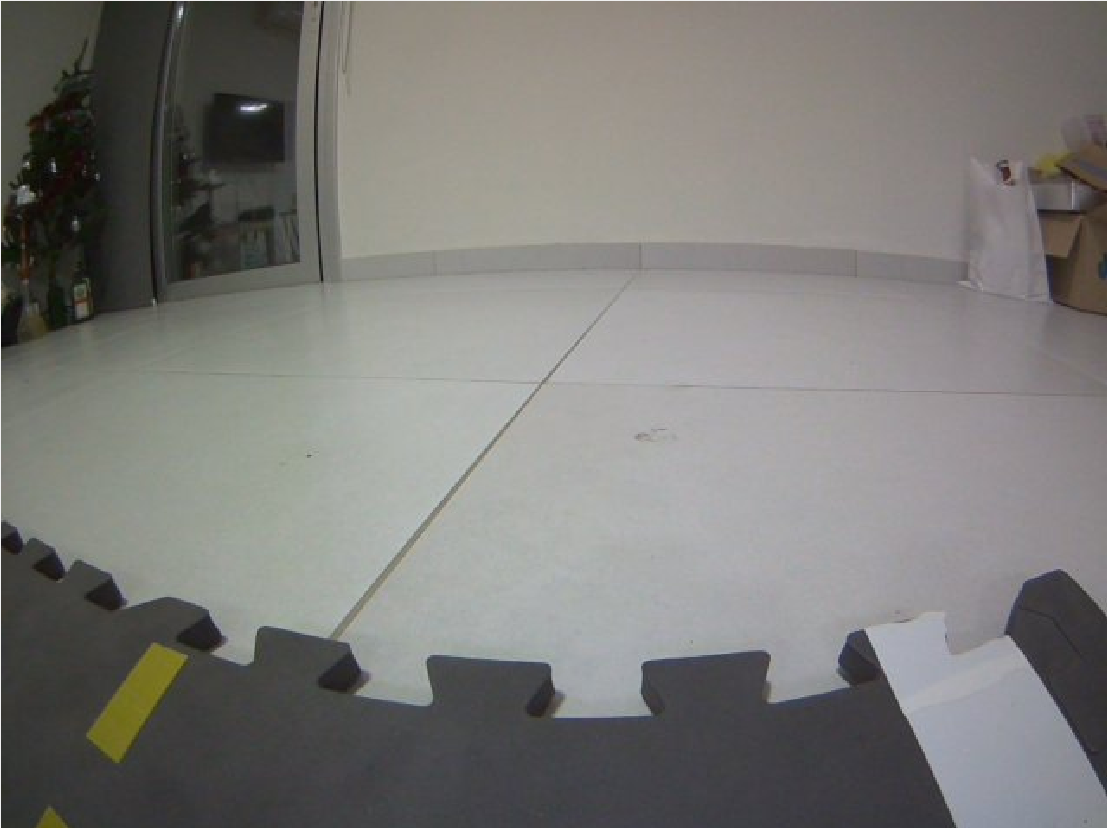
\includegraphics[scale=0.1]{src/EvaluationConclusionsAndFutureWork/assets/masks02.png}}
    \subfloat[Mask of the road with floor]{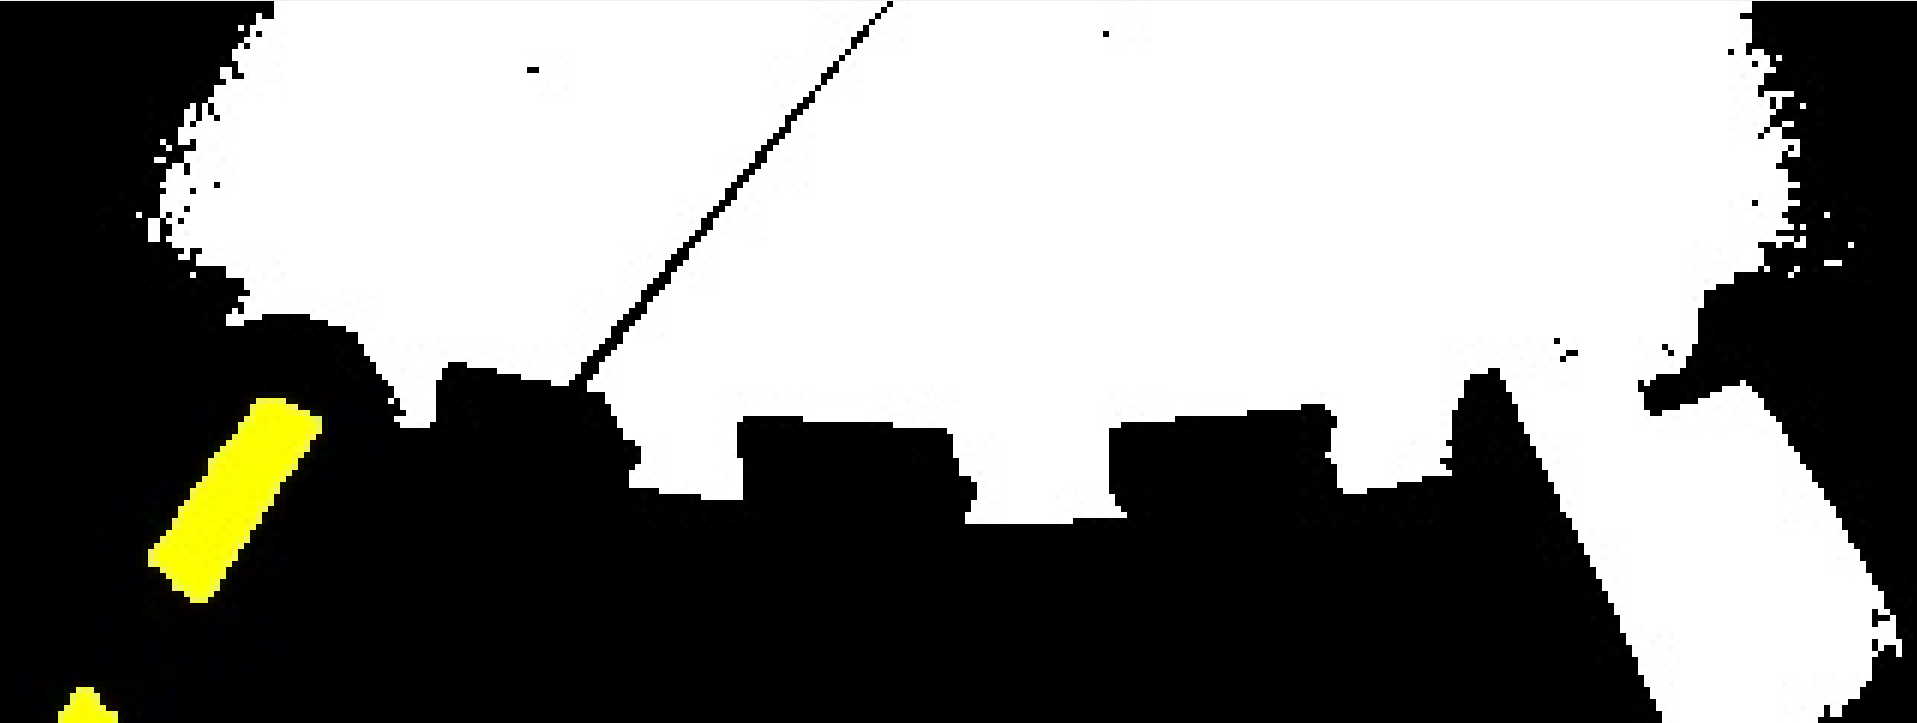
\includegraphics[scale=0.1]{src/EvaluationConclusionsAndFutureWork/assets/masks01.png}}
    \\
    \subfloat[Raw image of the road without floor]{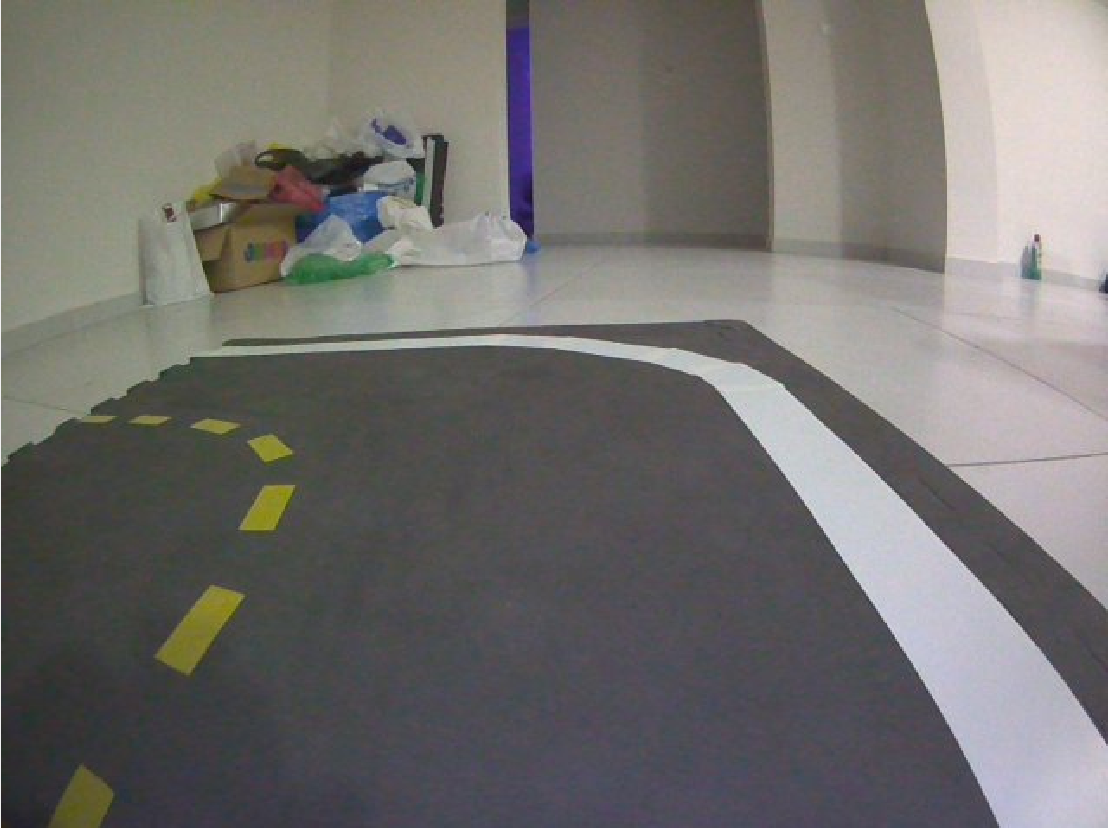
\includegraphics[scale=0.1]{src/EvaluationConclusionsAndFutureWork/assets/mask3.png}}
    \subfloat[Mask of the road without floor]{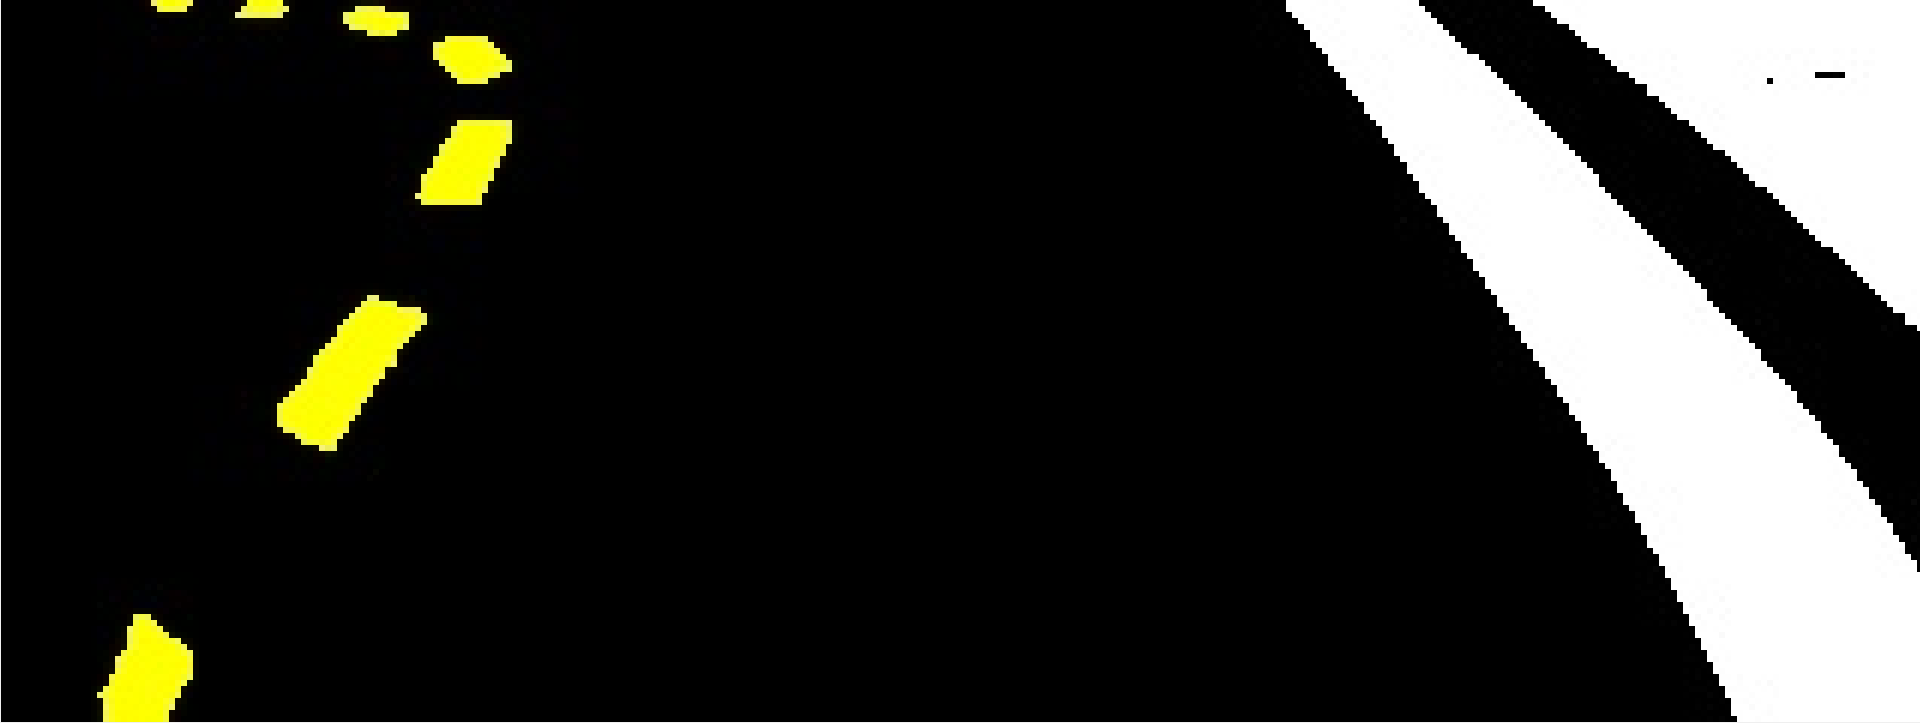
\includegraphics[scale=0.1]{src/EvaluationConclusionsAndFutureWork/assets/mask4.png}}
    \caption{Masks for different parts of the road}\label{fig:masks}
\end{figure}
\subsection{Applicability of Findings to the Commercial World}
This project is a research project, so it can't be directly applied in the commercial world. However, I've managed to create a good algorithm and collect a
pretty huge and well-marked dataset, which can help in developing the Duckietown project. Also, my contribution can help me find a job in computer vision, 
especially in self-driving car fields. 
\subsection{Conclusion}
As a result of the project the dataset was collected, marked up and published and the algorithm was created, deployed and published.
I've learned a few new things, like working with Docker or creating soft for robots. This project inspired me to dive into the world of reinforcement learning
to be able to create not only computer vision algorithms but also algorithms like autonomous lane following. The project was interesting and complicated, 
sometimes boring. But overall when Duckiebot finally drove by itself I was extremely happy.
\subsection{Future work}
Because of a lack of money for creating the polygon, I've decided to get rid of the red lines, which mark the beginning of the road intersection zone. So as future 
work adding a red line to the dataset can be considered. Also, these things can be done (and I'll probably do it, but not in the scope of this project):
\begin{enumerate}
    \item Combining my algorithm with the object detection algorithm. This step will fully close the lane-following problem because Duckiebot will be able to
    drive in the traffic lane, but also be able to detect objects (like duckies, which imitate pedestrians).
    \item Creating algorithm based on photogrammetry for crossing road intersection. This step in combination with the first one will fully solve the self-driving problem, 
    as the bot will be able to drive on any type of city road: basic road and traffic intersections.
    \item Improving lane following algorithm in the base image of Duckiebot.
    \item Create a driver for the Duckiebot camera so that it receives images immediately in the PyTorch-GPU-tensor format, so as not to waste time converting the tensor
    from CPU-tensor format to GPU-tensor. This driver can greatly speed up the work of computer vision algorithms on bots.
\end{enumerate}
